\documentclass{ali-presentation}

\title{Git and GitHub}
\subtitle{OI Orientation 2025}
\author{Alistair Pattison}

\usepackage{ulem}

\begin{document}

\begin{frame}
    \titlepage
\end{frame}

\section*{Why?}

\begin{frame}
    \frametitle{The State of OI}

    \begin{itemize}[<+->]
        \item ``Are you using using \texttt{fix\_incomes\_v\_55.py} or \texttt{fix\_incomes\_v\_54\_SI\_update\_final.py}?"
        \item ``Why is this result different ... I don't think I changed anything"
        \item ``\texttt{TODO: uncomment this later}"
        \item ``Wait that file was important??"
        \item ``I shouldn't delete this file it might be important later"
        \item ``Former predoc: Oh that file? It's in \texttt{old/archive/explore\_ishan}"
        \item ``Who is responsible for this line?"
    \end{itemize}

    \centering \bfseries \pause \color{red}

    These are not novel problems. \pause
    People have come up with a solution.

\end{frame}

\begin{frame}
    \frametitle{What is Git?}

    Git is...

    \pause \medskip
    
    \begin{quote}
        a fast, scalable, distributed revision control system with an unusually rich command set that provides both high-level operations and full access to internals.
        \normalfont -- the git manual
    \end{quote}

    \pause

    \begin{itemize}[<+->]
        \item Google Docs but for everything (code, papers, documentation, etc.)
        \item command-z on steroids
        \item a fully-reversable record of every change ever made in a codebase
        \item \sout{a} \emph{the} way for big groups to collaborate on big projects
    \end{itemize}
    
\end{frame}

\section{Using Git}

\begin{frame}
    \frametitle{Interacting with Git}

    \begin{enumerate}
        \item From the command line (e.g. \texttt{git pull}, \texttt{git clone})
        \begin{itemize}
            \item The original conception
            \item Far steeper learning curve, no visual feedback
            \item More control, faster once you get the hang of it
        \end{itemize}
        \bigskip \pause
        \item From some GUI (e.g. RStudio, VSCode, GitHub desktop)
        \begin{itemize}
            \item Easier to learn, visual feedback
            \item CS bros will judge you
            \pause
            \item \bfseries \color{red}Recommended for new users
        \end{itemize}
    \end{enumerate}

\end{frame}

\begin{frame}
    \frametitle{Aside: Working on Windows}

    \begin{itemize}
        \item Most tools for coding/software development are designed for Unix-based systems (Linux and Mac)
        \item Windows users can simulate Linux using WSL
        \item I recommend doing everything inside the Linux VM
        \begin{itemize}
            \item The WSL extension for VSCode extension makes this very easy
        \end{itemize}
    \end{itemize}

\end{frame}

\begin{frame}
    \frametitle{Practice workflow}

    \begin{enumerate}
        \item Download the codebase (\textit{clone} the \textit{repo})
        \begin{itemize}
            % \item \texttt{git clone https://github.com/opportunityinsights/git-practice} 
            \item In VSCode: source control tab $\rightarrow$ clone
        \end{itemize}
        \item Make your changes
        \begin{itemize}
            \item Fix the spelling of your name in \texttt{predocs.md}
        \end{itemize}
        \item Finalize your changes (\textit{commit} them)
        \begin{itemize}
            % \item \texttt{git commit -m 'fix Alistair's last name'}
            \item Click the plus, type a message, then click commit
        \end{itemize}
        \item Share your changes (\textit{push} to the remote)
        % \begin{itemize}
        %     \item \texttt{git push}
        % \end{itemize}
        \item Sync other people's changes (\textit{pull} from the remote)
        % \begin{itemize}
        %     \item \texttt{git pull}
        % \end{itemize}
    \end{enumerate}
\end{frame}

\begin{frame}
    \frametitle{Branches}

    \begin{itemize}[<+->]
        \item Allows you work on an isolated copy of the codebase (\texttt{git branch})
        \item Can easily switch between branches (\texttt{git switch})
        \item Merge your changes back into main branch (\texttt{git merge})
        \pause
        \begin{center}
            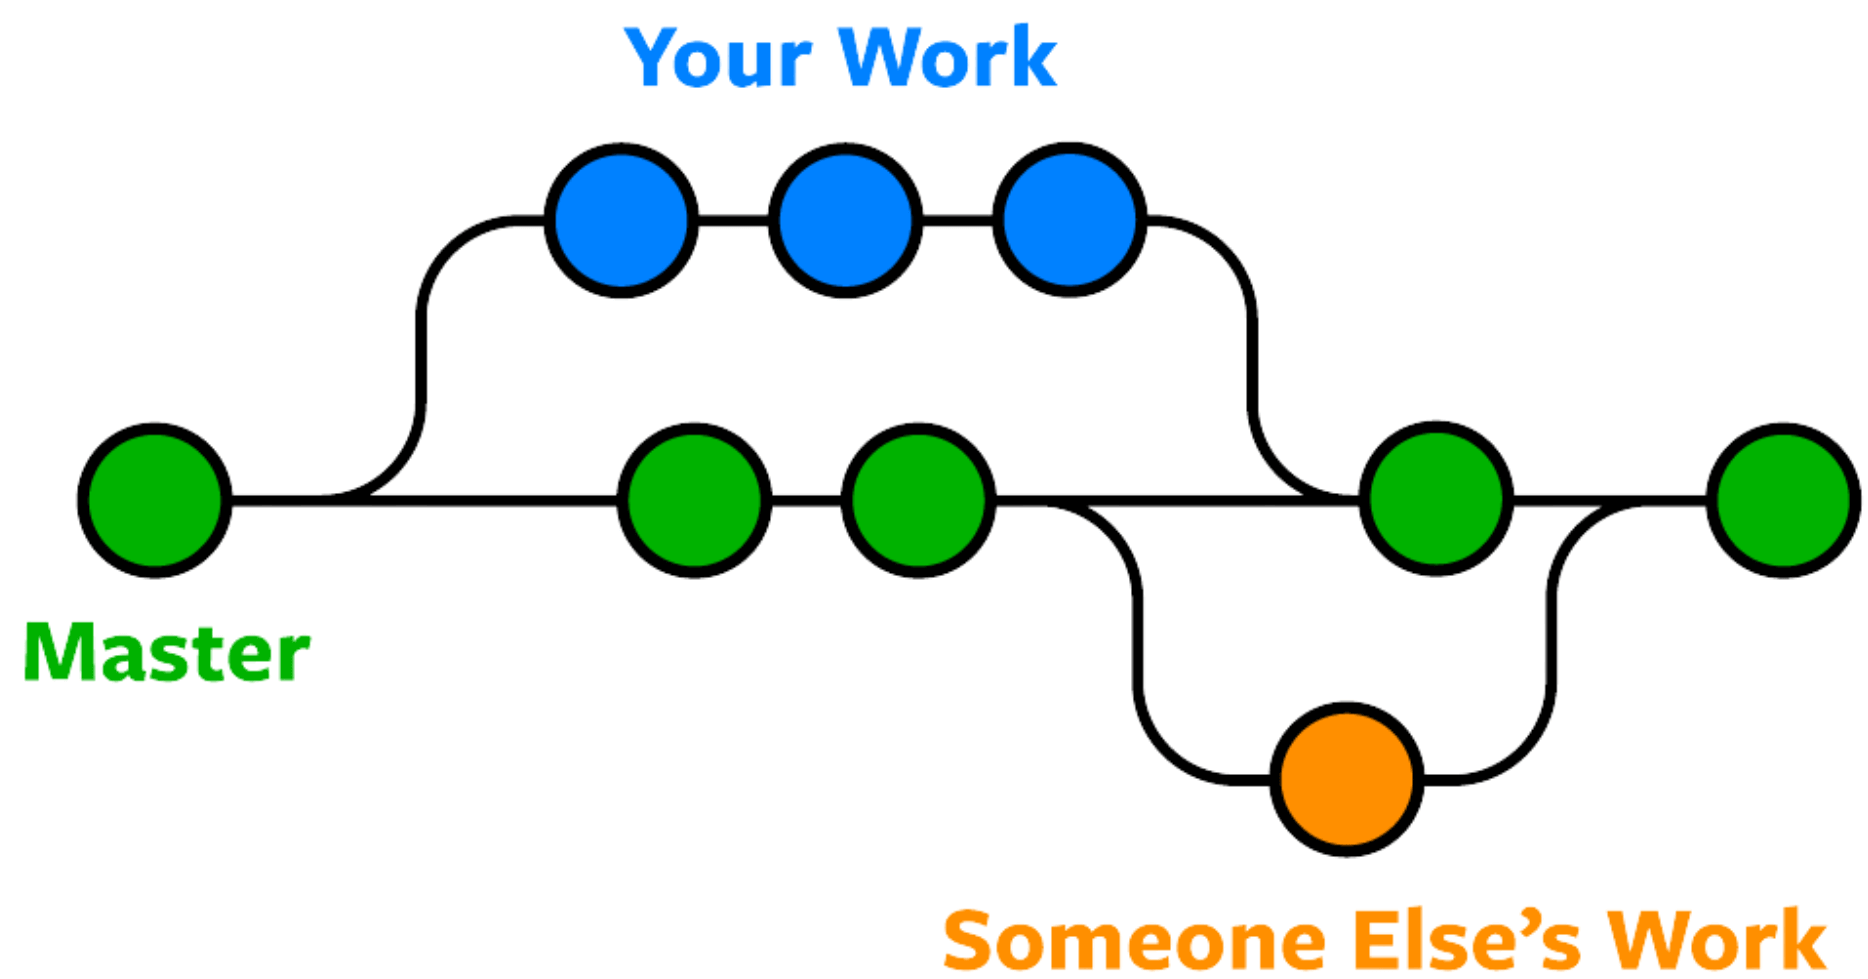
\includegraphics[width=.5\textwidth]{figures/branch.png}
        \end{center}
        \pause
        \item More info on this (and more) in the \href{https://code.visualstudio.com/docs/sourcecontrol/overview}{VSCode git documentation}
    \end{itemize}

\end{frame}

\begin{frame}
    \frametitle{Aside: Git in Census}

    There is a conception that Git is impossible on the inside.
    \pause
    This is \emph{\color{red} \textbf{FALSE}}.

    \bigskip \pause
    
    \begin{itemize}[<+->]
        \item Git exists
        \item VSCode exists (access with \texttt{qint \&\& code})
        \item It's the \emph{exact same process} (without pushing and pulling)
    \end{itemize}

\end{frame}

\begin{frame}
    \frametitle{Why not just use Dropbox?}
    
    \pause

    \textbf{Cop-out answer:}
    Because literally every company worth its salt uses some kind of version control and it would be moronic of us to ignore decades of established best-practices.

    \pause

    \textbf{Real answer}
    \begin{itemize}[<+->]
        \item Multiple people can edit at once
        \item Branches enable multiple people to work on different things
        \item Produces ``diffs" (compare codebase to previous state)
        \item Can roll back individual changes that occured far in the past
        \begin{itemize}
            \item \texttt{git revert}
        \end{itemize}
        \item Can opt out of tracking certain files via a \texttt{.gitignore}
    \end{itemize}

    \pause

    \tiny{Michael also has opinions: \url{https://michaelstepner.com/blog/git-vs-dropbox/}}

\end{frame}

\section{GitHub}

\begin{frame}
    \frametitle{Git vs. GitHub}

    \textbf{Git}

    \begin{itemize}
        \item Runs locally on your computer
        \item Keeps track of changes and branches
        \item Open source, old AF (2005!)
    \end{itemize}

    \pause

    \textbf{GitHub}

    \begin{itemize}
        \item A platform for remotely hosting git repositories 
        \item Provides wraparound features (e.g. pull requests, issues, wiki, etc.)
        \item Owned by Microsoft, but free* to use
    \end{itemize}
\end{frame}

\begin{frame}
    \frametitle{OI GitHub}

    \textbf{Project-specific}

    \begin{itemize}
        \item Health: \texttt{opportunityinsights/health-inequality}
        \item Credit: \texttt{opportunityinsights/credit}
    \end{itemize}

    \pause
    
    \textbf{General}

    \begin{itemize}
        \item Predoc wiki: \texttt{opportunityinsights/predoc-handbook}
        \item OI ggplot theme: \texttt{opportunityinsights/oiplot}
    \end{itemize}
\end{frame}

\begin{frame}
    \frametitle{Other GitHub Features}

    \begin{itemize}
        \item Permalinks (links to a specific line in a specific line in a specific file)
        \begin{itemize}
            \item E.g. Hannes (collaborator) asked for code, I sent him \href{https://github.com/OpportunityInsights/finer_geos_outside/blob/be912a2cc52a9e24b9e94d9e4d0d0364b42ae4ea/replication_code/code/analysis/misc_oz_scalars.do\#L76}{this link}
            \item Click the three dots in the margin $\rightarrow$ ``copy permalink''
        \end{itemize}
        \item Wikis
        \begin{itemize}
            \item Convenient place to collect information related to a project
        \end{itemize}
        \item Pull requests
        \begin{itemize}
            \item PR = request to merge your code into someone else's repository
            \item E.g. \href{https://github.com/anishathalye/dotbot/pull/377}{this one} I made a few months ago
        \end{itemize}
        \item Organizations and sharing permissions
        \item Nice web interface
        \item Github actions
        \begin{itemize}
            \item Code that automatically runs e.g. every day at 5pm or on every push
        \end{itemize}
    \end{itemize}
\end{frame}

\begin{frame}
    \frametitle{Resources}

    \begin{itemize}
        \item These slides
        \item The VSCode Git documenation: \url{https://code.visualstudio.com/docs/sourcecontrol/overview}
        \item The Git book: \url{https://git-scm.com/book/en/v2}
        \item ChatGPT (quite good when you don't know what to google)
    \end{itemize}
    
\end{frame}

\end{document}
